\documentclass[]{book}
\usepackage{lmodern}
\usepackage{amssymb,amsmath}
\usepackage{ifxetex,ifluatex}
\usepackage{fixltx2e} % provides \textsubscript
\ifnum 0\ifxetex 1\fi\ifluatex 1\fi=0 % if pdftex
  \usepackage[T1]{fontenc}
  \usepackage[utf8]{inputenc}
\else % if luatex or xelatex
  \ifxetex
    \usepackage{mathspec}
  \else
    \usepackage{fontspec}
  \fi
  \defaultfontfeatures{Ligatures=TeX,Scale=MatchLowercase}
\fi
% use upquote if available, for straight quotes in verbatim environments
\IfFileExists{upquote.sty}{\usepackage{upquote}}{}
% use microtype if available
\IfFileExists{microtype.sty}{%
\usepackage{microtype}
\UseMicrotypeSet[protrusion]{basicmath} % disable protrusion for tt fonts
}{}
\usepackage{hyperref}
\hypersetup{unicode=true,
            pdftitle={HEADS 2nd semester},
            pdfauthor={Bruno A Lima},
            pdfborder={0 0 0},
            breaklinks=true}
\urlstyle{same}  % don't use monospace font for urls
\usepackage{natbib}
\bibliographystyle{apalike}
\usepackage{color}
\usepackage{fancyvrb}
\newcommand{\VerbBar}{|}
\newcommand{\VERB}{\Verb[commandchars=\\\{\}]}
\DefineVerbatimEnvironment{Highlighting}{Verbatim}{commandchars=\\\{\}}
% Add ',fontsize=\small' for more characters per line
\usepackage{framed}
\definecolor{shadecolor}{RGB}{248,248,248}
\newenvironment{Shaded}{\begin{snugshade}}{\end{snugshade}}
\newcommand{\AlertTok}[1]{\textcolor[rgb]{0.94,0.16,0.16}{#1}}
\newcommand{\AnnotationTok}[1]{\textcolor[rgb]{0.56,0.35,0.01}{\textbf{\textit{#1}}}}
\newcommand{\AttributeTok}[1]{\textcolor[rgb]{0.77,0.63,0.00}{#1}}
\newcommand{\BaseNTok}[1]{\textcolor[rgb]{0.00,0.00,0.81}{#1}}
\newcommand{\BuiltInTok}[1]{#1}
\newcommand{\CharTok}[1]{\textcolor[rgb]{0.31,0.60,0.02}{#1}}
\newcommand{\CommentTok}[1]{\textcolor[rgb]{0.56,0.35,0.01}{\textit{#1}}}
\newcommand{\CommentVarTok}[1]{\textcolor[rgb]{0.56,0.35,0.01}{\textbf{\textit{#1}}}}
\newcommand{\ConstantTok}[1]{\textcolor[rgb]{0.00,0.00,0.00}{#1}}
\newcommand{\ControlFlowTok}[1]{\textcolor[rgb]{0.13,0.29,0.53}{\textbf{#1}}}
\newcommand{\DataTypeTok}[1]{\textcolor[rgb]{0.13,0.29,0.53}{#1}}
\newcommand{\DecValTok}[1]{\textcolor[rgb]{0.00,0.00,0.81}{#1}}
\newcommand{\DocumentationTok}[1]{\textcolor[rgb]{0.56,0.35,0.01}{\textbf{\textit{#1}}}}
\newcommand{\ErrorTok}[1]{\textcolor[rgb]{0.64,0.00,0.00}{\textbf{#1}}}
\newcommand{\ExtensionTok}[1]{#1}
\newcommand{\FloatTok}[1]{\textcolor[rgb]{0.00,0.00,0.81}{#1}}
\newcommand{\FunctionTok}[1]{\textcolor[rgb]{0.00,0.00,0.00}{#1}}
\newcommand{\ImportTok}[1]{#1}
\newcommand{\InformationTok}[1]{\textcolor[rgb]{0.56,0.35,0.01}{\textbf{\textit{#1}}}}
\newcommand{\KeywordTok}[1]{\textcolor[rgb]{0.13,0.29,0.53}{\textbf{#1}}}
\newcommand{\NormalTok}[1]{#1}
\newcommand{\OperatorTok}[1]{\textcolor[rgb]{0.81,0.36,0.00}{\textbf{#1}}}
\newcommand{\OtherTok}[1]{\textcolor[rgb]{0.56,0.35,0.01}{#1}}
\newcommand{\PreprocessorTok}[1]{\textcolor[rgb]{0.56,0.35,0.01}{\textit{#1}}}
\newcommand{\RegionMarkerTok}[1]{#1}
\newcommand{\SpecialCharTok}[1]{\textcolor[rgb]{0.00,0.00,0.00}{#1}}
\newcommand{\SpecialStringTok}[1]{\textcolor[rgb]{0.31,0.60,0.02}{#1}}
\newcommand{\StringTok}[1]{\textcolor[rgb]{0.31,0.60,0.02}{#1}}
\newcommand{\VariableTok}[1]{\textcolor[rgb]{0.00,0.00,0.00}{#1}}
\newcommand{\VerbatimStringTok}[1]{\textcolor[rgb]{0.31,0.60,0.02}{#1}}
\newcommand{\WarningTok}[1]{\textcolor[rgb]{0.56,0.35,0.01}{\textbf{\textit{#1}}}}
\usepackage{longtable,booktabs}
\usepackage{graphicx,grffile}
\makeatletter
\def\maxwidth{\ifdim\Gin@nat@width>\linewidth\linewidth\else\Gin@nat@width\fi}
\def\maxheight{\ifdim\Gin@nat@height>\textheight\textheight\else\Gin@nat@height\fi}
\makeatother
% Scale images if necessary, so that they will not overflow the page
% margins by default, and it is still possible to overwrite the defaults
% using explicit options in \includegraphics[width, height, ...]{}
\setkeys{Gin}{width=\maxwidth,height=\maxheight,keepaspectratio}
\IfFileExists{parskip.sty}{%
\usepackage{parskip}
}{% else
\setlength{\parindent}{0pt}
\setlength{\parskip}{6pt plus 2pt minus 1pt}
}
\setlength{\emergencystretch}{3em}  % prevent overfull lines
\providecommand{\tightlist}{%
  \setlength{\itemsep}{0pt}\setlength{\parskip}{0pt}}
\setcounter{secnumdepth}{5}
% Redefines (sub)paragraphs to behave more like sections
\ifx\paragraph\undefined\else
\let\oldparagraph\paragraph
\renewcommand{\paragraph}[1]{\oldparagraph{#1}\mbox{}}
\fi
\ifx\subparagraph\undefined\else
\let\oldsubparagraph\subparagraph
\renewcommand{\subparagraph}[1]{\oldsubparagraph{#1}\mbox{}}
\fi

%%% Use protect on footnotes to avoid problems with footnotes in titles
\let\rmarkdownfootnote\footnote%
\def\footnote{\protect\rmarkdownfootnote}

%%% Change title format to be more compact
\usepackage{titling}

% Create subtitle command for use in maketitle
\providecommand{\subtitle}[1]{
  \posttitle{
    \begin{center}\large#1\end{center}
    }
}

\setlength{\droptitle}{-2em}

  \title{HEADS 2nd semester}
    \pretitle{\vspace{\droptitle}\centering\huge}
  \posttitle{\par}
    \author{Bruno A Lima}
    \preauthor{\centering\large\emph}
  \postauthor{\par}
      \predate{\centering\large\emph}
  \postdate{\par}
    \date{2020-02-10}

\usepackage{booktabs}

\begin{document}
\maketitle

{
\setcounter{tocdepth}{1}
\tableofcontents
}
\hypertarget{section}{%
\chapter*{}\label{section}}
\addcontentsline{toc}{chapter}{}


\includegraphics{images/heads.png}

\hypertarget{preface}{%
\chapter*{Preface}\label{preface}}
\addcontentsline{toc}{chapter}{Preface}

This is a \emph{book} written in \textbf{Markdown} through \emph{RStudio}.

The \textbf{bookdown} package \citep{xie2015} can be installed from CRAN or Github:

\begin{Shaded}
\begin{Highlighting}[]
\KeywordTok{install.packages}\NormalTok{(}\StringTok{"bookdown"}\NormalTok{)}
\CommentTok{# or the development version}
\CommentTok{# devtools::install_github("rstudio/bookdown")}
\end{Highlighting}
\end{Shaded}

In this \emph{book}, I will try to compile all the homeworks from the 2nd semester 2019/2020 of \textbf{HEADS} PhD programme.

An exhaustive explanation using the \textbf{bookdown} package \citep{R-bookdown} can be found at bookdown: Authoring Books and Technical Documents with R Markdown and this is only a sample book, which was built on top of R Markdown and \textbf{knitr}

This \emph{book} is publish through NETLIFY as described by C.M.

\hypertarget{intro}{%
\chapter{Introduction}\label{intro}}

All the files and code of this book are available in the repository: \url{https://github.com/balima78/HEADS2sem}.

All the students can contribute to this compilation sending me their own homeworks and correcting the mistakes I will certainly do. You can send me your files and code to \texttt{balima78@gmail.com}. When possible you must send me \emph{.Rmd} files and data as \emph{.csv}.

Here, \emph{.Rmd} files are named by number from 1000 to 9000 (\textbf{CLLS} - \textbf{C}lass \textbf{LL}esson \textbf{S}tudent) followed by a breave description.

You can label chapter and section titles using \texttt{\{\#label\}} after them, e.g., we can reference Chapter \ref{top}. If you do not manually label them, there will be automatic labels anyway, e.g., Chapter \ref{compstat}.

Figures and tables with captions will be placed in \texttt{figure} and \texttt{table} environments, respectively.

\begin{Shaded}
\begin{Highlighting}[]
\KeywordTok{par}\NormalTok{(}\DataTypeTok{mar =} \KeywordTok{c}\NormalTok{(}\DecValTok{4}\NormalTok{, }\DecValTok{4}\NormalTok{, }\FloatTok{.1}\NormalTok{, }\FloatTok{.1}\NormalTok{))}
\KeywordTok{plot}\NormalTok{(pressure, }\DataTypeTok{type =} \StringTok{'b'}\NormalTok{, }\DataTypeTok{pch =} \DecValTok{19}\NormalTok{)}
\end{Highlighting}
\end{Shaded}

\begin{figure}

{\centering 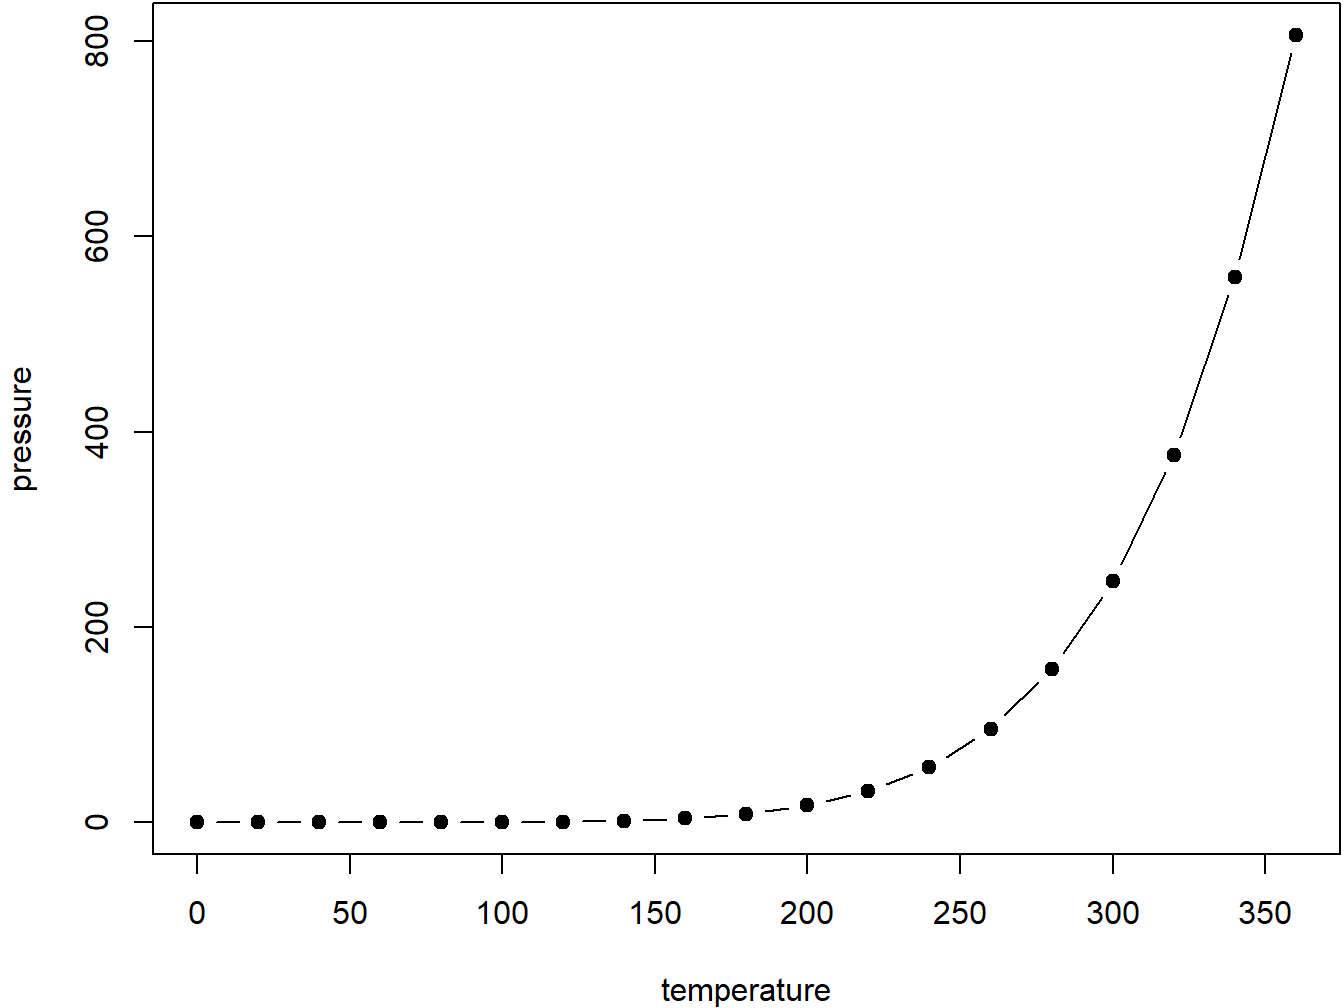
\includegraphics[width=0.8\linewidth]{heads2sem_files/figure-latex/nice-fig-1} 

}

\caption{Here is a nice figure!}\label{fig:nice-fig}
\end{figure}

Reference a figure by its code chunk label with the \texttt{fig:} prefix, e.g., see Figure \ref{fig:nice-fig}. Similarly, you can reference tables generated from \texttt{knitr::kable()}, e.g., see Table \ref{tab:nice-tab}.

\begin{Shaded}
\begin{Highlighting}[]
\NormalTok{knitr}\OperatorTok{::}\KeywordTok{kable}\NormalTok{(}
  \KeywordTok{head}\NormalTok{(iris, }\DecValTok{6}\NormalTok{), }\DataTypeTok{caption =} \StringTok{'Here is a nice table!'}\NormalTok{,}
  \DataTypeTok{booktabs =} \OtherTok{TRUE}
\NormalTok{)}
\end{Highlighting}
\end{Shaded}

\begin{table}

\caption{\label{tab:nice-tab}Here is a nice table!}
\centering
\begin{tabular}[t]{rrrrl}
\toprule
Sepal.Length & Sepal.Width & Petal.Length & Petal.Width & Species\\
\midrule
5.1 & 3.5 & 1.4 & 0.2 & setosa\\
4.9 & 3.0 & 1.4 & 0.2 & setosa\\
4.7 & 3.2 & 1.3 & 0.2 & setosa\\
4.6 & 3.1 & 1.5 & 0.2 & setosa\\
5.0 & 3.6 & 1.4 & 0.2 & setosa\\
\addlinespace
5.4 & 3.9 & 1.7 & 0.4 & setosa\\
\bottomrule
\end{tabular}
\end{table}

You can write citations, too. For example, we are using the \textbf{bookdown} package \citep{R-bookdown} in this sample book, which was built on top of R Markdown and \textbf{knitr} \citep{xie2015}.

\hypertarget{compstat}{%
\chapter{COMPSTAT}\label{compstat}}

\emph{Estatística Computacional}

\textbf{Conteúdos programáticos}

Estatística computacional

\begin{itemize}
\tightlist
\item
  Porque usar computação em estatística?
\item
  Ferramentas e software para estatística computacional
\item
  Estatística computacional utilizando grandes infra-estruturas de dados
\end{itemize}

Sinopses de dados

\begin{itemize}
\tightlist
\item
  Estatísticas suficientes
\item
  Histogramas
\item
  Micro-Clusters
\item
  Fading Statistics
\end{itemize}

Estimativas de densidade

\begin{itemize}
\tightlist
\item
  Máxima verosimilhança
\item
  Expectation-Maximization
\item
  Kernel Estimation
\end{itemize}

Estimativas e Simulação

\begin{itemize}
\tightlist
\item
  Métodos Jackknife
\item
  Validação cruzada
\item
  Geração de números aleatórios
\item
  Métodos de Monte Carlo
\item
  Métodos de Bootstrap
\end{itemize}

Análise numérica

\begin{itemize}
\tightlist
\item
  Visualização de dados complexos
\item
  Análise de componentes principais
\item
  Bivariate smoothing
\item
  Splines
\end{itemize}

\hypertarget{lesson-1}{%
\section{Lesson 1}\label{lesson-1}}

2020-02-03

\textbf{Exercises Solutions} (just copied teacher's solutions)

\begin{enumerate}
\def\labelenumi{\arabic{enumi}.}
\tightlist
\item
  Open the database Anesthesia-BD.csv
\end{enumerate}

\begin{Shaded}
\begin{Highlighting}[]
\NormalTok{data =}\StringTok{ }\KeywordTok{read.csv}\NormalTok{(}\StringTok{"2.UploadedData/Anesthesia-BD.csv"}\NormalTok{) }\CommentTok{###load dat}

\KeywordTok{str}\NormalTok{(data) }\CommentTok{###see data structure}
\end{Highlighting}
\end{Shaded}

\begin{verbatim}
## 'data.frame':    387 obs. of  9 variables:
##  $ Subject         : Factor w/ 387 levels "Sbj001","Sbj002",..: 1 2 3 4 5 6 7 8 9 10 ...
##  $ Gender          : Factor w/ 2 levels "Female","Male": 2 2 1 2 2 2 2 2 2 1 ...
##  $ Age             : int  50 67 71 51 69 78 70 58 80 63 ...
##  $ TypeSurgery     : Factor w/ 3 levels "CAB","CAB + Valve",..: 3 1 1 3 1 2 1 3 3 2 ...
##  $ SurgStatus      : Factor w/ 2 levels "Elective","Urgent": 1 1 2 1 2 2 1 2 1 2 ...
##  $ Diastolic       : num  45.5 52.6 56.7 71.4 58.1 ...
##  $ Systolic        : num  112.1 109 98.2 150.8 131.5 ...
##  $ Cross_Clamp_Time: int  83 67 83 51 63 114 94 138 42 172 ...
##  $ AdvEvent        : int  0 0 0 0 1 0 0 0 0 0 ...
\end{verbatim}

Factor variable AdvEvent

\begin{Shaded}
\begin{Highlighting}[]
\NormalTok{data}\OperatorTok{$}\NormalTok{AdvEvent <-}\StringTok{ }\KeywordTok{factor}\NormalTok{(data}\OperatorTok{$}\NormalTok{AdvEvent, }\DataTypeTok{levels =} \KeywordTok{c}\NormalTok{(}\DecValTok{0}\NormalTok{,}\DecValTok{1}\NormalTok{),}\DataTypeTok{labels=}\KeywordTok{c}\NormalTok{(}\StringTok{"No"}\NormalTok{,}\StringTok{"Yes"}\NormalTok{))}
\end{Highlighting}
\end{Shaded}

\begin{enumerate}
\def\labelenumi{\arabic{enumi}.}
\setcounter{enumi}{1}
\tightlist
\item
  For the columns which contain numeric values, create a new summary table in which the rows are the mean, the standard deviation, and the median of each of the numeric columns.
\end{enumerate}

\begin{Shaded}
\begin{Highlighting}[]
\NormalTok{T <-}\StringTok{ }\KeywordTok{sapply}\NormalTok{(data[,}\KeywordTok{sapply}\NormalTok{(data,is.numeric)],}\ControlFlowTok{function}\NormalTok{(x)\{}
  \KeywordTok{return}\NormalTok{(}\KeywordTok{rbind}\NormalTok{(}\KeywordTok{mean}\NormalTok{(x,}\DataTypeTok{na.rm =}\NormalTok{ T),}\KeywordTok{sd}\NormalTok{(x,}\DataTypeTok{na.rm =}\NormalTok{ T),}\KeywordTok{median}\NormalTok{(x,}\DataTypeTok{na.rm =}\NormalTok{ T)))}
\NormalTok{  \}}
\NormalTok{  )}

\KeywordTok{rownames}\NormalTok{(T) =}\StringTok{ }\KeywordTok{c}\NormalTok{(}\StringTok{"Mean"}\NormalTok{,}\StringTok{"SD"}\NormalTok{,}\StringTok{"Median"}\NormalTok{)}

\NormalTok{T}
\end{Highlighting}
\end{Shaded}

\begin{verbatim}
##             Age Diastolic  Systolic Cross_Clamp_Time
## Mean   67.27390  60.93076 132.04705         72.00521
## SD     11.25574  11.35387  21.22864         32.04680
## Median 67.00000  60.52591 130.00410         67.00000
\end{verbatim}

\begin{enumerate}
\def\labelenumi{\arabic{enumi}.}
\setcounter{enumi}{2}
\tightlist
\item
  Considering only the subjects who had CAB or Valve surgery, how many had adverse events? How many males and females in the two groups (having or not having adverse events)? (count and percentage)
\end{enumerate}

\begin{Shaded}
\begin{Highlighting}[]
\CommentTok{# create an index with the observation that comply with the conditions}
\NormalTok{ind =}\StringTok{ }\KeywordTok{which}\NormalTok{(data}\OperatorTok{$}\NormalTok{TypeSurgery}\OperatorTok{==}\StringTok{"CAB"} \OperatorTok{|}\StringTok{ }\NormalTok{data}\OperatorTok{$}\NormalTok{TypeSurgery}\OperatorTok{==}\StringTok{"Valve"}\NormalTok{ )}

\CommentTok{# table these data counts}
\KeywordTok{table}\NormalTok{(data[ind,}\StringTok{"AdvEvent"}\NormalTok{])}
\end{Highlighting}
\end{Shaded}

\begin{verbatim}
## 
##  No Yes 
## 231  80
\end{verbatim}

\begin{Shaded}
\begin{Highlighting}[]
\CommentTok{# and frequencies}
\KeywordTok{prop.table}\NormalTok{(}\KeywordTok{table}\NormalTok{(data[ind,}\StringTok{"AdvEvent"}\NormalTok{]))}
\end{Highlighting}
\end{Shaded}

\begin{verbatim}
## 
##        No       Yes 
## 0.7427653 0.2572347
\end{verbatim}

\begin{Shaded}
\begin{Highlighting}[]
\CommentTok{# now by gender}
\KeywordTok{table}\NormalTok{(data[ind,}\StringTok{"Gender"}\NormalTok{],data[ind,}\StringTok{"AdvEvent"}\NormalTok{])}
\end{Highlighting}
\end{Shaded}

\begin{verbatim}
##         
##           No Yes
##   Female  60  21
##   Male   171  59
\end{verbatim}

\begin{Shaded}
\begin{Highlighting}[]
\CommentTok{# and their frequencies}
\KeywordTok{prop.table}\NormalTok{(}\KeywordTok{table}\NormalTok{(data[ind,}\StringTok{"Gender"}\NormalTok{],data[ind,}\StringTok{"AdvEvent"}\NormalTok{]))}
\end{Highlighting}
\end{Shaded}

\begin{verbatim}
##         
##                  No        Yes
##   Female 0.19292605 0.06752412
##   Male   0.54983923 0.18971061
\end{verbatim}

4.Merge the two datasets (Anesthesia-BD.csv and Anesthesia-BD2.csv)
by the subject identification number.

\begin{Shaded}
\begin{Highlighting}[]
\NormalTok{data2 =}\StringTok{ }\KeywordTok{read.csv}\NormalTok{(}\StringTok{"2.UploadedData/Anesthesia-BD2.csv"}\NormalTok{) }\CommentTok{###load data Anesthesia-BD2.csv}

\CommentTok{# I had to rename the first column, I don't know why}
\KeywordTok{names}\NormalTok{(data2)[}\DecValTok{1}\NormalTok{]<-}\StringTok{"SubjectID"}

\KeywordTok{str}\NormalTok{(data2)}
\end{Highlighting}
\end{Shaded}

\begin{verbatim}
## 'data.frame':    363 obs. of  7 variables:
##  $ SubjectID         : Factor w/ 363 levels "Sbj001","Sbj002",..: 3 25 30 32 36 39 46 56 60 63 ...
##  $ Diabetes          : int  0 0 1 1 0 0 0 1 0 0 ...
##  $ RFLastA1cLevel    : num  5.7 5.6 7.1 6.7 6.7 6.3 6 6.5 5.3 4.9 ...
##  $ ChronicLungDisease: Factor w/ 4 levels "Mild","Moderate",..: 1 1 1 1 1 1 1 1 1 1 ...
##  $ Hypertension      : int  1 1 1 1 1 1 1 1 1 1 ...
##  $ CHF               : int  0 1 1 1 1 1 1 0 1 1 ...
##  $ Euroscore         : Factor w/ 330 levels "#N/A","0.501743134",..: 8 64 4 92 249 36 195 125 214 224 ...
\end{verbatim}

\begin{enumerate}
\def\labelenumi{\Alph{enumi})}
\tightlist
\item
  The merge must be such that only the common subjects should be present in the final database (natural join).
\end{enumerate}

\begin{Shaded}
\begin{Highlighting}[]
\NormalTok{Ma =}\StringTok{ }\KeywordTok{merge}\NormalTok{(data,data2,}\DataTypeTok{by.x =} \StringTok{"Subject"}\NormalTok{,}\DataTypeTok{by.y=}\StringTok{"SubjectID"}\NormalTok{,}\DataTypeTok{all =}\NormalTok{ F)}

\KeywordTok{dim}\NormalTok{(Ma)}
\end{Highlighting}
\end{Shaded}

\begin{verbatim}
## [1] 363  15
\end{verbatim}

\begin{enumerate}
\def\labelenumi{\Alph{enumi})}
\setcounter{enumi}{1}
\tightlist
\item
  The merge must be such that if some subject is not in one of the databases, the subject should be in the database, and missing information must be not available (full outer join).
\end{enumerate}

\begin{Shaded}
\begin{Highlighting}[]
\NormalTok{Mb =}\StringTok{ }\KeywordTok{merge}\NormalTok{(data,data2,}\DataTypeTok{by.x =} \StringTok{"Subject"}\NormalTok{,}\DataTypeTok{by.y=}\StringTok{"SubjectID"}\NormalTok{,}\DataTypeTok{all =}\NormalTok{ T)}

\KeywordTok{dim}\NormalTok{(Mb)}
\end{Highlighting}
\end{Shaded}

\begin{verbatim}
## [1] 387  15
\end{verbatim}

Consider the following statement: ``For people without diabetes, the normal range for the hemoglobin A1c level is between 4\% and 5.6\%. Hemoglobin A1c levels between 5.7\% and 6.4\% mean you have a higher chance of getting diabetes. Levels of 6.5\% or higher mean you have diabetes.''

\begin{enumerate}
\def\labelenumi{\arabic{enumi}.}
\setcounter{enumi}{4}
\tightlist
\item
  Create a new variable with three factors (normal, prediabetes, and diabetes), taking into consideration the values the A1c levels. Compare the results obtained with the variable Diabetes (assuming that 1 means to have diabetes and 0 no diabetes).
\end{enumerate}

\begin{Shaded}
\begin{Highlighting}[]
\NormalTok{diab <-}\StringTok{ }\KeywordTok{ifelse}\NormalTok{(Mb}\OperatorTok{$}\NormalTok{RFLastA1cLevel}\OperatorTok{<}\FloatTok{5.7}\NormalTok{,}\DecValTok{0}\NormalTok{,}\KeywordTok{ifelse}\NormalTok{(Mb}\OperatorTok{$}\NormalTok{RFLastA1cLevel}\OperatorTok{<}\FloatTok{6.4}\NormalTok{,}\DecValTok{1}\NormalTok{,}\DecValTok{2}\NormalTok{))}

\NormalTok{Mb}\OperatorTok{$}\NormalTok{Diabetes2 <-}\StringTok{ }\KeywordTok{factor}\NormalTok{(}\DataTypeTok{x =}\NormalTok{ diab,}
                       \DataTypeTok{levels =} \DecValTok{0}\OperatorTok{:}\DecValTok{2}\NormalTok{, }
                       \DataTypeTok{labels =}\KeywordTok{c}\NormalTok{(}\StringTok{"Normal"}\NormalTok{,}\StringTok{"PreDiabetes"}\NormalTok{,}\StringTok{"Diabetes"}\NormalTok{))}

\NormalTok{Mb}\OperatorTok{$}\NormalTok{Diabetes <-}\StringTok{ }\KeywordTok{factor}\NormalTok{(Mb}\OperatorTok{$}\NormalTok{Diabetes,}
                      \DataTypeTok{levels=}\DecValTok{0}\OperatorTok{:}\DecValTok{1}\NormalTok{,}
                      \DataTypeTok{labels=}\KeywordTok{c}\NormalTok{(}\StringTok{"Normal"}\NormalTok{,}\StringTok{"Diabetes"}\NormalTok{))}

\KeywordTok{table}\NormalTok{(Mb}\OperatorTok{$}\NormalTok{Diabetes,Mb}\OperatorTok{$}\NormalTok{Diabetes2)}
\end{Highlighting}
\end{Shaded}

\begin{verbatim}
##           
##            Normal PreDiabetes Diabetes
##   Normal      120          99       11
##   Diabetes      7          35       83
\end{verbatim}

\begin{enumerate}
\def\labelenumi{\arabic{enumi}.}
\setcounter{enumi}{5}
\tightlist
\item
  Create a table with the comparison between the groups having or not having
  adverse events for all the variables available in the combined database. Use the
  appropriate measures for each type of variable.
\end{enumerate}

\begin{Shaded}
\begin{Highlighting}[]
\KeywordTok{str}\NormalTok{(Mb)}
\end{Highlighting}
\end{Shaded}

\begin{verbatim}
## 'data.frame':    387 obs. of  16 variables:
##  $ Subject           : Factor w/ 387 levels "Sbj001","Sbj002",..: 1 2 3 4 5 6 7 8 9 10 ...
##  $ Gender            : Factor w/ 2 levels "Female","Male": 2 2 1 2 2 2 2 2 2 1 ...
##  $ Age               : int  50 67 71 51 69 78 70 58 80 63 ...
##  $ TypeSurgery       : Factor w/ 3 levels "CAB","CAB + Valve",..: 3 1 1 3 1 2 1 3 3 2 ...
##  $ SurgStatus        : Factor w/ 2 levels "Elective","Urgent": 1 1 2 1 2 2 1 2 1 2 ...
##  $ Diastolic         : num  45.5 52.6 56.7 71.4 58.1 ...
##  $ Systolic          : num  112.1 109 98.2 150.8 131.5 ...
##  $ Cross_Clamp_Time  : int  83 67 83 51 63 114 94 138 42 172 ...
##  $ AdvEvent          : Factor w/ 2 levels "No","Yes": 1 1 1 1 2 1 1 1 1 1 ...
##  $ Diabetes          : Factor w/ 2 levels "Normal","Diabetes": 2 1 1 1 1 1 1 1 1 2 ...
##  $ RFLastA1cLevel    : num  7.9 5.5 5.7 6 5.8 NA 5.9 6 5.2 11.2 ...
##  $ ChronicLungDisease: Factor w/ 4 levels "Mild","Moderate",..: 3 3 1 3 3 3 3 3 3 3 ...
##  $ Hypertension      : int  1 1 1 0 1 0 1 1 1 0 ...
##  $ CHF               : int  1 0 0 0 0 1 1 1 1 1 ...
##  $ Euroscore         : Factor w/ 330 levels "#N/A","0.501743134",..: 47 206 8 289 159 96 119 98 77 4 ...
##  $ Diabetes2         : Factor w/ 3 levels "Normal","PreDiabetes",..: 3 1 2 2 2 NA 2 2 1 3 ...
\end{verbatim}

\begin{Shaded}
\begin{Highlighting}[]
\NormalTok{Mb}\OperatorTok{$}\NormalTok{Hypertension <-}\StringTok{ }\KeywordTok{factor}\NormalTok{(Mb}\OperatorTok{$}\NormalTok{Hypertension,}
                          \DataTypeTok{levels=}\DecValTok{0}\OperatorTok{:}\DecValTok{1}\NormalTok{,}
                          \DataTypeTok{labels=}\KeywordTok{c}\NormalTok{(}\StringTok{"No"}\NormalTok{,}\StringTok{"Yes"}\NormalTok{))}

\NormalTok{Mb}\OperatorTok{$}\NormalTok{CHF <-}\StringTok{ }\KeywordTok{factor}\NormalTok{(Mb}\OperatorTok{$}\NormalTok{CHF,}
                 \DataTypeTok{levels=}\DecValTok{0}\OperatorTok{:}\DecValTok{1}\NormalTok{,}
                 \DataTypeTok{labels=}\KeywordTok{c}\NormalTok{(}\StringTok{"No"}\NormalTok{,}\StringTok{"Yes"}\NormalTok{))}

\NormalTok{Mb}\OperatorTok{$}\NormalTok{Subject <-}\StringTok{ }\KeywordTok{as.character}\NormalTok{(Mb}\OperatorTok{$}\NormalTok{Subject)}

\CommentTok{#windows()}

\KeywordTok{par}\NormalTok{(}\DataTypeTok{mfrow=}\KeywordTok{c}\NormalTok{(}\DecValTok{2}\NormalTok{,}\DecValTok{3}\NormalTok{))}

\ControlFlowTok{for}\NormalTok{ (i }\ControlFlowTok{in} \KeywordTok{which}\NormalTok{(}\KeywordTok{sapply}\NormalTok{(Mb,is.numeric)))\{}
\KeywordTok{hist}\NormalTok{(Mb[,i],}\DataTypeTok{xlab=}\KeywordTok{colnames}\NormalTok{(Mb)[i])}
\NormalTok{\}}

\KeywordTok{par}\NormalTok{(}\DataTypeTok{mfrow=}\KeywordTok{c}\NormalTok{(}\DecValTok{1}\NormalTok{,}\DecValTok{1}\NormalTok{))}
\end{Highlighting}
\end{Shaded}

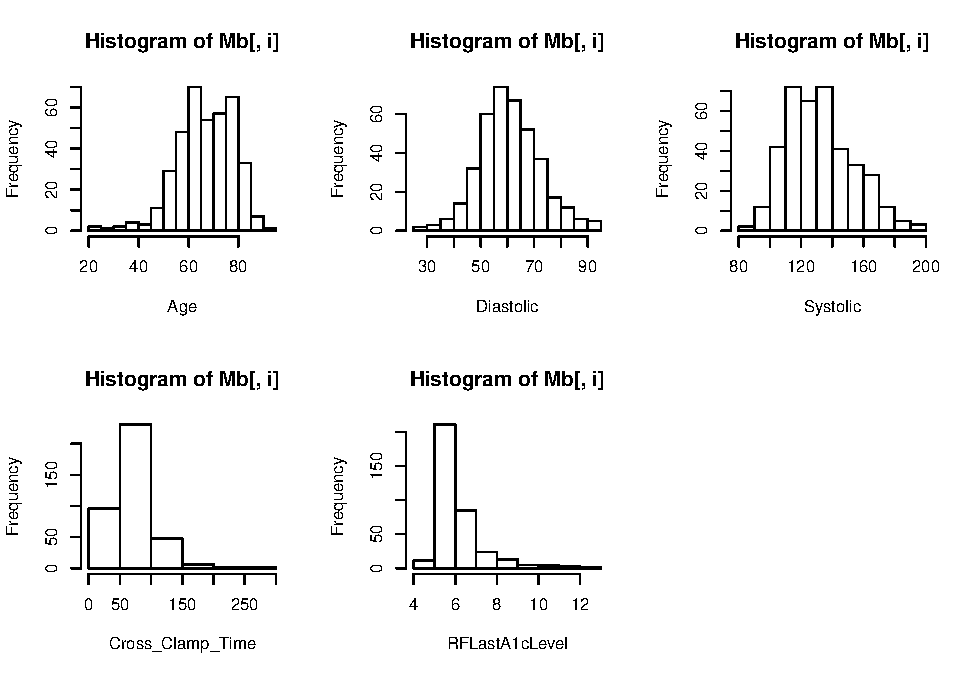
\includegraphics{heads2sem_files/figure-latex/unnamed-chunk-17-1.pdf}

\begin{Shaded}
\begin{Highlighting}[]
\NormalTok{table <-}\StringTok{ }\KeywordTok{by}\NormalTok{(Mb[,}\KeywordTok{which}\NormalTok{(}\KeywordTok{sapply}\NormalTok{(Mb,is.numeric))],}
            \DataTypeTok{INDICES =}\NormalTok{ Mb}\OperatorTok{$}\NormalTok{AdvEvent,}
            \DataTypeTok{FUN =} \ControlFlowTok{function}\NormalTok{(x) }\KeywordTok{apply}\NormalTok{(x,}\DecValTok{2}\NormalTok{,quantile,}\DataTypeTok{na.rm=}\NormalTok{T))}

\NormalTok{table}
\end{Highlighting}
\end{Shaded}

\begin{verbatim}
## Mb$AdvEvent: No
##      Age Diastolic  Systolic Cross_Clamp_Time RFLastA1cLevel
## 0%    25  26.42047  88.70903               15            4.7
## 25%   59  53.30694 115.03977               51            5.6
## 50%   67  60.75382 129.50300               68            5.8
## 75%   76  68.64874 143.12238               83            6.4
## 100%  92  94.35495 180.95547              241           12.2
## -------------------------------------------------------- 
## Mb$AdvEvent: Yes
##      Age Diastolic  Systolic Cross_Clamp_Time RFLastA1cLevel
## 0%    24  39.42266  92.34727             13.0          4.600
## 25%   62  52.93295 119.55877             48.0          5.500
## 50%   69  59.94571 131.48461             64.0          5.800
## 75%   77  65.97349 153.50990             88.5          6.425
## 100%  88  92.51766 193.75080            298.0         11.700
\end{verbatim}

\begin{Shaded}
\begin{Highlighting}[]
\NormalTok{table}\OperatorTok{$}\NormalTok{pvalue <-}\StringTok{ }\KeywordTok{apply}\NormalTok{(Mb[,}\KeywordTok{which}\NormalTok{(}\KeywordTok{sapply}\NormalTok{(Mb,is.numeric))],}\DecValTok{2}\NormalTok{,}
                      \ControlFlowTok{function}\NormalTok{(x)}
                        \KeywordTok{wilcox.test}\NormalTok{(x[}\KeywordTok{which}\NormalTok{(Mb}\OperatorTok{$}\NormalTok{AdvEvent}\OperatorTok{==}\StringTok{"No"}\NormalTok{)],x[}\KeywordTok{which}\NormalTok{(Mb}\OperatorTok{$}\NormalTok{AdvEvent}\OperatorTok{==}\StringTok{"Yes"}\NormalTok{)])}\OperatorTok{$}\NormalTok{p.value)}

\NormalTok{table}
\end{Highlighting}
\end{Shaded}

\begin{verbatim}
##      Age Diastolic  Systolic Cross_Clamp_Time RFLastA1cLevel
## 0%    25  26.42047  88.70903               15            4.7
## 25%   59  53.30694 115.03977               51            5.6
## 50%   67  60.75382 129.50300               68            5.8
## 75%   76  68.64874 143.12238               83            6.4
## 100%  92  94.35495 180.95547              241           12.2
## -------------------------------------------------------- 
##      Age Diastolic  Systolic Cross_Clamp_Time RFLastA1cLevel
## 0%    24  39.42266  92.34727             13.0          4.600
## 25%   62  52.93295 119.55877             48.0          5.500
## 50%   69  59.94571 131.48461             64.0          5.800
## 75%   77  65.97349 153.50990             88.5          6.425
## 100%  88  92.51766 193.75080            298.0         11.700
## -------------------------------------------------------- 
##              Age        Diastolic         Systolic Cross_Clamp_Time 
##       0.09297764       0.41375034       0.09079886       0.76575185 
##   RFLastA1cLevel 
##       0.78804579
\end{verbatim}

\begin{Shaded}
\begin{Highlighting}[]
\NormalTok{Mb}\OperatorTok{$}\NormalTok{Euroscore<-}\KeywordTok{as.character}\NormalTok{(Mb}\OperatorTok{$}\NormalTok{Euroscore)}

\NormalTok{table2 <-}\StringTok{ }\KeywordTok{by}\NormalTok{(Mb[,}\KeywordTok{which}\NormalTok{(}\KeywordTok{sapply}\NormalTok{(Mb,is.factor))], }
             \DataTypeTok{INDICES =}\NormalTok{ Mb}\OperatorTok{$}\NormalTok{AdvEvent, }
             \DataTypeTok{FUN =} \ControlFlowTok{function}\NormalTok{(x)\{}\KeywordTok{sapply}\NormalTok{(x,table)\})}

\NormalTok{table2}
\end{Highlighting}
\end{Shaded}

\begin{verbatim}
## Mb$AdvEvent: No
## $Gender
## 
## Female   Male 
##     78    200 
## 
## $TypeSurgery
## 
##         CAB CAB + Valve       Valve 
##         156          47          75 
## 
## $SurgStatus
## 
## Elective   Urgent 
##      148      130 
## 
## $AdvEvent
## 
##  No Yes 
## 278   0 
## 
## $Diabetes
## 
##   Normal Diabetes 
##      170       93 
## 
## $ChronicLungDisease
## 
##     Mild Moderate       No   Severe 
##       34        4      226        1 
## 
## $Hypertension
## 
##  No Yes 
##  49 215 
## 
## $CHF
## 
##  No Yes 
## 186  79 
## 
## $Diabetes2
## 
##      Normal PreDiabetes    Diabetes 
##          91         100          70 
## 
## -------------------------------------------------------- 
## Mb$AdvEvent: Yes
## $Gender
## 
## Female   Male 
##     31     78 
## 
## $TypeSurgery
## 
##         CAB CAB + Valve       Valve 
##          41          29          39 
## 
## $SurgStatus
## 
## Elective   Urgent 
##       64       45 
## 
## $AdvEvent
## 
##  No Yes 
##   0 109 
## 
## $Diabetes
## 
##   Normal Diabetes 
##       65       33 
## 
## $ChronicLungDisease
## 
##     Mild Moderate       No   Severe 
##       16        0       79        3 
## 
## $Hypertension
## 
##  No Yes 
##  20  78 
## 
## $CHF
## 
##  No Yes 
##  50  47 
## 
## $Diabetes2
## 
##      Normal PreDiabetes    Diabetes 
##          36          35          25
\end{verbatim}

\hypertarget{stats}{%
\chapter{STATS}\label{stats}}

\emph{Modelação Estatística}

\textbf{Conteúdos programáticos}

\begin{itemize}
\tightlist
\item
  Regressão logística.
\item
  Análise de sobrevivência.
\item
  Análise de dados longitudinais.
\item
  Causalidade.
\end{itemize}

\hypertarget{learn}{%
\chapter{LEARN}\label{learn}}

\emph{Macine Learning}

\textbf{Conteúdos programáticos}

O processo de extração de conhecimento de dados

\begin{itemize}
\tightlist
\item
  Compreensão do negócio
\item
  Compreensão dos dados
\item
  Pré-processamento de dados
\item
  Modelação de dados
\item
  Avaliação de modelos de extração de conhecimento de dados
\item
  Implantação prática dos resultados de modelação
\end{itemize}

Aprendizagem automática

\begin{itemize}
\tightlist
\item
  Aprender conceitos a partir de dados
\item
  Processos indutivos vs processos dedutivos
\item
  Viés indutivo
\item
  Validação de modelos
\item
  Medidas de erro e processos de estimação
\end{itemize}

Aprendizagem supervisionada

\begin{itemize}
\tightlist
\item
  Árvores de decisão
\item
  Redes Bayesianas
\item
  Redes neuronais
\item
  Deep learning e análise de grandes bases de dados
\end{itemize}

Aprendizagem não supervisionada

\begin{itemize}
\tightlist
\item
  Análise de clusters
\item
  Deteção de casos extremos e anomalias
\item
  Associação e análise de padrões frequentes
\item
  Interpretação de grandes bases de dados
\end{itemize}

\hypertarget{lesson-1-1}{%
\section{Lesson 1}\label{lesson-1-1}}

2020-02-04

This exercise was done as described by: \url{https://machinelearningmastery.com/machine-learning-in-r-step-by-step/}

but using a data set from:
\url{https://archive.ics.uci.edu/ml/datasets/Breast+Cancer+Coimbra\#}

Read the data

\begin{Shaded}
\begin{Highlighting}[]
\NormalTok{dataset <-}\StringTok{ }\KeywordTok{read.csv}\NormalTok{(}\StringTok{"2.UploadedData/dataR2.csv"}\NormalTok{)}
\end{Highlighting}
\end{Shaded}

Factor variable \emph{Classification}

\begin{Shaded}
\begin{Highlighting}[]
\NormalTok{dataset}\OperatorTok{$}\NormalTok{Classification<-}\KeywordTok{as.factor}\NormalTok{(dataset}\OperatorTok{$}\NormalTok{Classification)}
\end{Highlighting}
\end{Shaded}

\textbf{NOTE}: in order to use the caret packages in all its' capabilities you must do \texttt{install.packages("caret",\ dependencies\ =\ T)}

create a validation dataset and use the remaing for training

\begin{Shaded}
\begin{Highlighting}[]
\KeywordTok{library}\NormalTok{(caret)}

\CommentTok{# create a list of 80% of the rows in the original dataset we can use for training}
\NormalTok{validation_index <-}\StringTok{ }\KeywordTok{createDataPartition}\NormalTok{(dataset}\OperatorTok{$}\NormalTok{Classification, }\DataTypeTok{p=}\FloatTok{0.80}\NormalTok{, }\DataTypeTok{list=}\OtherTok{FALSE}\NormalTok{)}
\CommentTok{# select 20% of the data for validation}
\NormalTok{validation <-}\StringTok{ }\NormalTok{dataset[}\OperatorTok{-}\NormalTok{validation_index,]}
\CommentTok{# use the remaining 80% of data to training and testing the models}
\NormalTok{dataset <-}\StringTok{ }\NormalTok{dataset[validation_index,]}
\end{Highlighting}
\end{Shaded}

dimensions of the new dataset

\begin{Shaded}
\begin{Highlighting}[]
\KeywordTok{dim}\NormalTok{(dataset)}
\end{Highlighting}
\end{Shaded}

\begin{verbatim}
## [1] 94 10
\end{verbatim}

list types for each attribute

\begin{Shaded}
\begin{Highlighting}[]
\KeywordTok{sapply}\NormalTok{(dataset, class)}
\end{Highlighting}
\end{Shaded}

\begin{verbatim}
##            Age            BMI        Glucose        Insulin           HOMA 
##      "integer"      "numeric"      "integer"      "numeric"      "numeric" 
##         Leptin    Adiponectin       Resistin          MCP.1 Classification 
##      "numeric"      "numeric"      "numeric"      "numeric"       "factor"
\end{verbatim}

take a peek at the first 5 rows of the data

\begin{Shaded}
\begin{Highlighting}[]
\KeywordTok{head}\NormalTok{(dataset)}
\end{Highlighting}
\end{Shaded}

\begin{verbatim}
##   Age      BMI Glucose Insulin      HOMA Leptin Adiponectin Resistin
## 1  48 23.50000      70   2.707 0.4674087 8.8071    9.702400  7.99585
## 2  83 20.69049      92   3.115 0.7068973 8.8438    5.429285  4.06405
## 4  68 21.36752      77   3.226 0.6127249 9.8827    7.169560 12.76600
## 5  86 21.11111      92   3.549 0.8053864 6.6994    4.819240 10.57635
## 6  49 22.85446      92   3.226 0.7320869 6.8317   13.679750 10.31760
## 8  76 23.80000     118   6.470 1.8832013 4.3110   13.251320  5.10420
##     MCP.1 Classification
## 1 417.114              1
## 2 468.786              1
## 4 928.220              1
## 5 773.920              1
## 6 530.410              1
## 8 280.694              1
\end{verbatim}

list the levels for the class

\begin{Shaded}
\begin{Highlighting}[]
\KeywordTok{levels}\NormalTok{(dataset}\OperatorTok{$}\NormalTok{Classification)}
\end{Highlighting}
\end{Shaded}

\begin{verbatim}
## [1] "1" "2"
\end{verbatim}

summarize the class distribution

\begin{Shaded}
\begin{Highlighting}[]
\NormalTok{percentage <-}\StringTok{ }\KeywordTok{prop.table}\NormalTok{(}\KeywordTok{table}\NormalTok{(dataset}\OperatorTok{$}\NormalTok{Classification)) }\OperatorTok{*}\StringTok{ }\DecValTok{100}
\KeywordTok{cbind}\NormalTok{(}\DataTypeTok{freq=}\KeywordTok{table}\NormalTok{(dataset}\OperatorTok{$}\NormalTok{Classification), }\DataTypeTok{percentage=}\NormalTok{percentage)}
\end{Highlighting}
\end{Shaded}

\begin{verbatim}
##   freq percentage
## 1   42   44.68085
## 2   52   55.31915
\end{verbatim}

summarize attribute distributions

\begin{Shaded}
\begin{Highlighting}[]
\KeywordTok{summary}\NormalTok{(dataset)}
\end{Highlighting}
\end{Shaded}

\begin{verbatim}
##       Age             BMI           Glucose          Insulin      
##  Min.   :24.00   Min.   :18.37   Min.   : 60.00   Min.   : 2.432  
##  1st Qu.:45.00   1st Qu.:23.04   1st Qu.: 86.00   1st Qu.: 4.111  
##  Median :55.50   Median :27.66   Median : 93.00   Median : 5.906  
##  Mean   :57.11   Mean   :27.67   Mean   : 98.96   Mean   :10.019  
##  3rd Qu.:70.50   3rd Qu.:31.24   3rd Qu.:103.00   3rd Qu.:10.539  
##  Max.   :86.00   Max.   :38.58   Max.   :201.00   Max.   :58.460  
##       HOMA             Leptin        Adiponectin        Resistin     
##  Min.   : 0.4674   Min.   : 4.311   Min.   : 1.656   Min.   : 3.210  
##  1st Qu.: 0.8319   1st Qu.:12.309   1st Qu.: 5.438   1st Qu.: 6.745  
##  Median : 1.3775   Median :19.587   Median : 8.208   Median :10.636  
##  Mean   : 2.7538   Mean   :26.081   Mean   :10.202   Mean   :14.800  
##  3rd Qu.: 2.6293   3rd Qu.:34.983   3rd Qu.:11.872   3rd Qu.:17.067  
##  Max.   :25.0503   Max.   :89.270   Max.   :38.040   Max.   :82.100  
##      MCP.1         Classification
##  Min.   :  45.84   1:42          
##  1st Qu.: 257.88   2:52          
##  Median : 412.16                 
##  Mean   : 519.76                 
##  3rd Qu.: 702.68                 
##  Max.   :1698.44
\end{verbatim}

split input and output

\begin{Shaded}
\begin{Highlighting}[]
\NormalTok{x <-}\StringTok{ }\NormalTok{dataset[,}\DecValTok{1}\OperatorTok{:}\DecValTok{9}\NormalTok{]}
\NormalTok{y <-}\StringTok{ }\NormalTok{dataset[,}\DecValTok{10}\NormalTok{]}
\end{Highlighting}
\end{Shaded}

boxplot for each attribute on one image

\begin{Shaded}
\begin{Highlighting}[]
\KeywordTok{par}\NormalTok{(}\DataTypeTok{mfrow=}\KeywordTok{c}\NormalTok{(}\DecValTok{2}\NormalTok{,}\DecValTok{5}\NormalTok{))}
\ControlFlowTok{for}\NormalTok{(i }\ControlFlowTok{in} \DecValTok{1}\OperatorTok{:}\DecValTok{9}\NormalTok{) \{}
  \KeywordTok{boxplot}\NormalTok{(x[,i], }\DataTypeTok{main=}\KeywordTok{names}\NormalTok{(dataset)[i])}
\NormalTok{\}}
\end{Highlighting}
\end{Shaded}

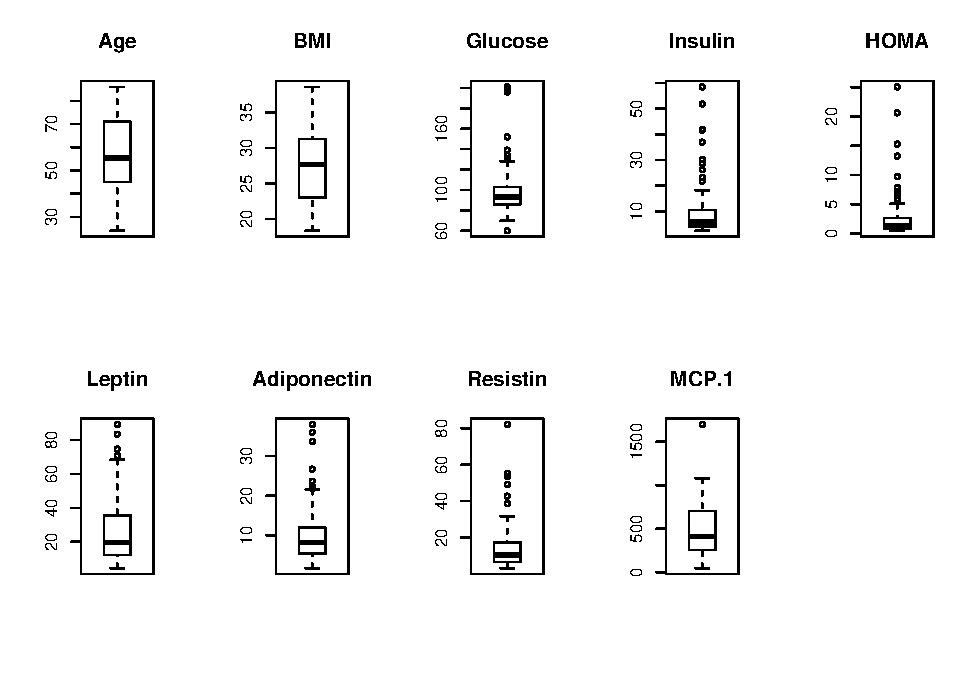
\includegraphics{heads2sem_files/figure-latex/unnamed-chunk-32-1.pdf}

barplot for class breakdown

\begin{Shaded}
\begin{Highlighting}[]
\KeywordTok{par}\NormalTok{(}\DataTypeTok{mfrow=}\KeywordTok{c}\NormalTok{(}\DecValTok{1}\NormalTok{,}\DecValTok{1}\NormalTok{))}

\KeywordTok{plot}\NormalTok{(y)}
\end{Highlighting}
\end{Shaded}

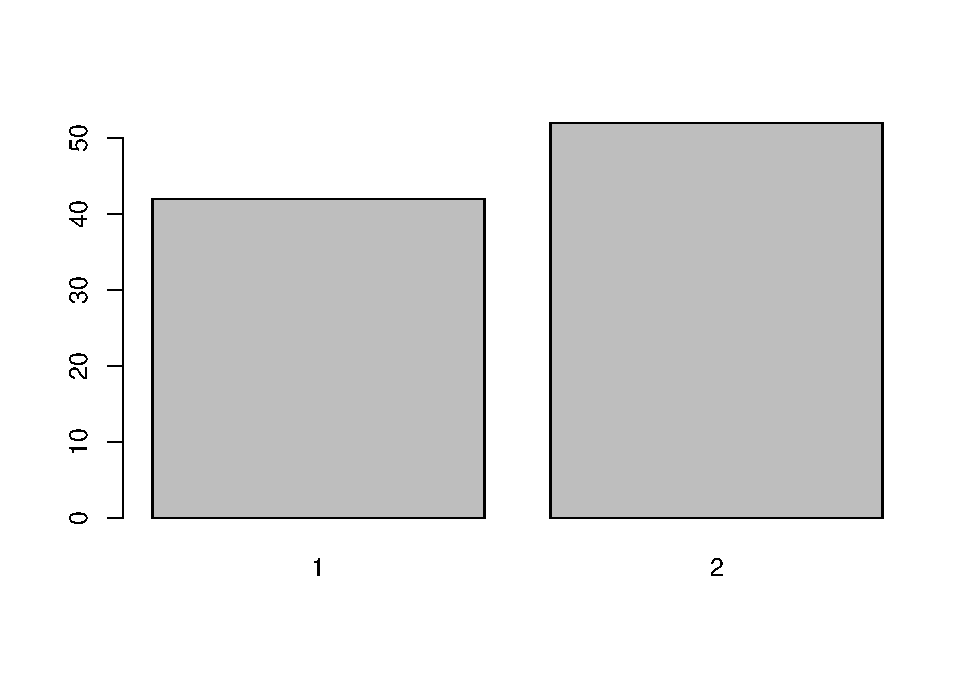
\includegraphics{heads2sem_files/figure-latex/unnamed-chunk-33-1.pdf}

scatterplot matrix

\begin{Shaded}
\begin{Highlighting}[]
\KeywordTok{featurePlot}\NormalTok{(}\DataTypeTok{x=}\NormalTok{x, }\DataTypeTok{y=}\NormalTok{y, }\DataTypeTok{plot=}\StringTok{"ellipse"}\NormalTok{)}
\end{Highlighting}
\end{Shaded}

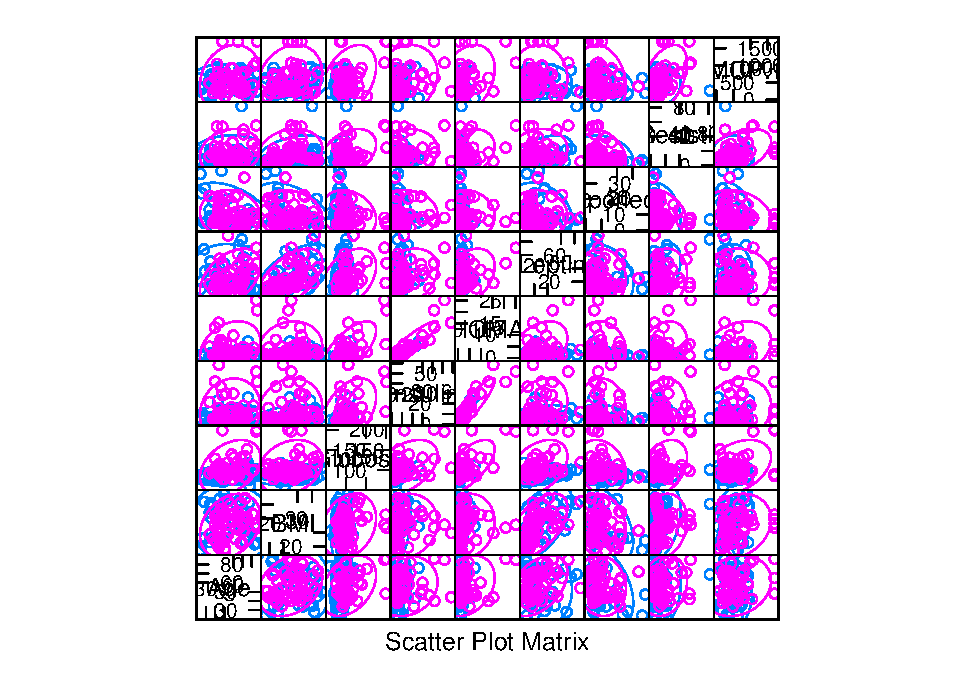
\includegraphics{heads2sem_files/figure-latex/unnamed-chunk-34-1.pdf}

box and whisker plots for each attribute

\begin{Shaded}
\begin{Highlighting}[]
\KeywordTok{featurePlot}\NormalTok{(}\DataTypeTok{x=}\NormalTok{x, }\DataTypeTok{y=}\NormalTok{y, }\DataTypeTok{plot=}\StringTok{"box"}\NormalTok{)}
\end{Highlighting}
\end{Shaded}

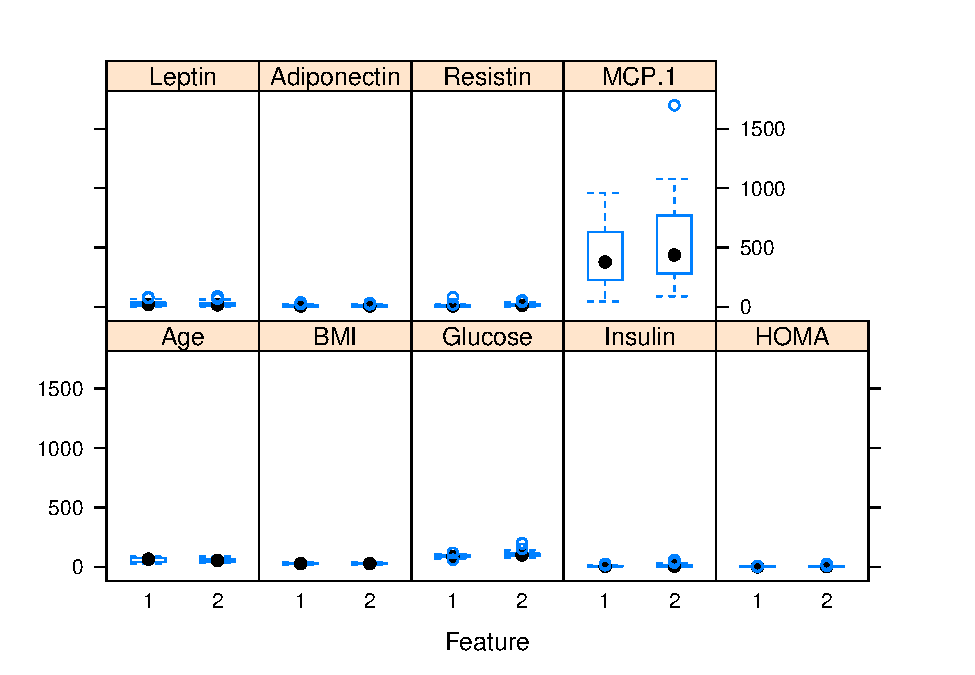
\includegraphics{heads2sem_files/figure-latex/unnamed-chunk-35-1.pdf}

density plots for each attribute by class value

\begin{Shaded}
\begin{Highlighting}[]
\NormalTok{scales <-}\StringTok{ }\KeywordTok{list}\NormalTok{(}\DataTypeTok{x=}\KeywordTok{list}\NormalTok{(}\DataTypeTok{relation=}\StringTok{"free"}\NormalTok{), }\DataTypeTok{y=}\KeywordTok{list}\NormalTok{(}\DataTypeTok{relation=}\StringTok{"free"}\NormalTok{))}
\KeywordTok{featurePlot}\NormalTok{(}\DataTypeTok{x=}\NormalTok{x, }\DataTypeTok{y=}\NormalTok{y, }\DataTypeTok{plot=}\StringTok{"density"}\NormalTok{, }\DataTypeTok{scales=}\NormalTok{scales)}
\end{Highlighting}
\end{Shaded}

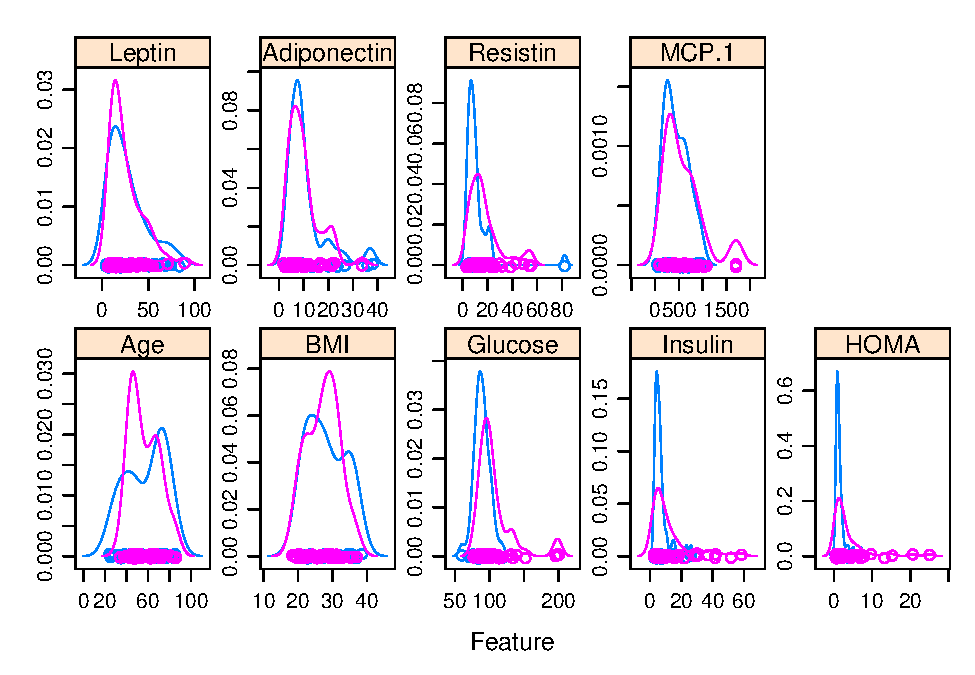
\includegraphics{heads2sem_files/figure-latex/unnamed-chunk-36-1.pdf}

Run algorithms using 10-fold cross validation

\begin{Shaded}
\begin{Highlighting}[]
\NormalTok{control <-}\StringTok{ }\KeywordTok{trainControl}\NormalTok{(}\DataTypeTok{method=}\StringTok{"cv"}\NormalTok{, }\DataTypeTok{number=}\DecValTok{10}\NormalTok{)}
\NormalTok{metric <-}\StringTok{ "Accuracy"}
\end{Highlighting}
\end{Shaded}

\begin{enumerate}
\def\labelenumi{\alph{enumi})}
\tightlist
\item
  linear algorithms
\end{enumerate}

\begin{Shaded}
\begin{Highlighting}[]
\KeywordTok{set.seed}\NormalTok{(}\DecValTok{7}\NormalTok{)}
\NormalTok{fit.lda <-}\StringTok{ }\KeywordTok{train}\NormalTok{(Classification}\OperatorTok{~}\NormalTok{., }\DataTypeTok{data=}\NormalTok{dataset, }\DataTypeTok{method=}\StringTok{"lda"}\NormalTok{, }\DataTypeTok{metric=}\NormalTok{metric, }\DataTypeTok{trControl=}\NormalTok{control)}
\end{Highlighting}
\end{Shaded}

\begin{enumerate}
\def\labelenumi{\alph{enumi})}
\setcounter{enumi}{1}
\tightlist
\item
  nonlinear algorithms
  CART
\end{enumerate}

\begin{Shaded}
\begin{Highlighting}[]
\KeywordTok{set.seed}\NormalTok{(}\DecValTok{7}\NormalTok{)}
\NormalTok{fit.cart <-}\StringTok{ }\KeywordTok{train}\NormalTok{(Classification}\OperatorTok{~}\NormalTok{., }\DataTypeTok{data=}\NormalTok{dataset, }\DataTypeTok{method=}\StringTok{"rpart"}\NormalTok{, }\DataTypeTok{metric=}\NormalTok{metric, }\DataTypeTok{trControl=}\NormalTok{control)}
\end{Highlighting}
\end{Shaded}

kNN

\begin{Shaded}
\begin{Highlighting}[]
\KeywordTok{set.seed}\NormalTok{(}\DecValTok{7}\NormalTok{)}
\NormalTok{fit.knn <-}\StringTok{ }\KeywordTok{train}\NormalTok{(Classification}\OperatorTok{~}\NormalTok{., }\DataTypeTok{data=}\NormalTok{dataset, }\DataTypeTok{method=}\StringTok{"knn"}\NormalTok{, }\DataTypeTok{metric=}\NormalTok{metric, }\DataTypeTok{trControl=}\NormalTok{control)}
\end{Highlighting}
\end{Shaded}

\begin{enumerate}
\def\labelenumi{\alph{enumi})}
\setcounter{enumi}{2}
\tightlist
\item
  advanced algorithms
  SVM
\end{enumerate}

\begin{Shaded}
\begin{Highlighting}[]
\KeywordTok{set.seed}\NormalTok{(}\DecValTok{7}\NormalTok{)}
\NormalTok{fit.svm <-}\StringTok{ }\KeywordTok{train}\NormalTok{(Classification}\OperatorTok{~}\NormalTok{., }\DataTypeTok{data=}\NormalTok{dataset, }\DataTypeTok{method=}\StringTok{"svmRadial"}\NormalTok{, }\DataTypeTok{metric=}\NormalTok{metric, }\DataTypeTok{trControl=}\NormalTok{control)}
\end{Highlighting}
\end{Shaded}

Random Forest

\begin{Shaded}
\begin{Highlighting}[]
\KeywordTok{set.seed}\NormalTok{(}\DecValTok{7}\NormalTok{)}
\NormalTok{fit.rf <-}\StringTok{ }\KeywordTok{train}\NormalTok{(Classification}\OperatorTok{~}\NormalTok{., }\DataTypeTok{data=}\NormalTok{dataset, }\DataTypeTok{method=}\StringTok{"rf"}\NormalTok{, }\DataTypeTok{metric=}\NormalTok{metric, }\DataTypeTok{trControl=}\NormalTok{control)}
\end{Highlighting}
\end{Shaded}

summarize accuracy of models

\begin{Shaded}
\begin{Highlighting}[]
\NormalTok{results <-}\StringTok{ }\KeywordTok{resamples}\NormalTok{(}\KeywordTok{list}\NormalTok{(}\DataTypeTok{lda=}\NormalTok{fit.lda, }\DataTypeTok{cart=}\NormalTok{fit.cart, }\DataTypeTok{knn=}\NormalTok{fit.knn, }\DataTypeTok{svm=}\NormalTok{fit.svm, }\DataTypeTok{rf=}\NormalTok{fit.rf))}
\KeywordTok{summary}\NormalTok{(results)}
\end{Highlighting}
\end{Shaded}

\begin{verbatim}
## 
## Call:
## summary.resamples(object = results)
## 
## Models: lda, cart, knn, svm, rf 
## Number of resamples: 10 
## 
## Accuracy 
##           Min.   1st Qu.    Median      Mean   3rd Qu.      Max. NA's
## lda  0.4000000 0.4722222 0.6277778 0.6786869 0.8888889 1.0000000    0
## cart 0.2222222 0.4444444 0.5000000 0.5030303 0.5555556 0.7777778    0
## knn  0.2222222 0.4583333 0.5505051 0.5312121 0.6500000 0.7777778    0
## svm  0.5555556 0.5833333 0.7500000 0.7540404 0.8712121 1.0000000    0
## rf   0.5000000 0.5757576 0.6833333 0.7169697 0.8611111 1.0000000    0
## 
## Kappa 
##             Min.    1st Qu.     Median         Mean   3rd Qu.      Max.
## lda  -0.15384615 -0.1022267 0.27142857  0.349208393 0.7692308 1.0000000
## cart -0.61538462 -0.1270125 0.00000000 -0.002034517 0.1000000 0.5500000
## knn  -0.53658537 -0.1153846 0.06754386  0.047012771 0.2807692 0.5263158
## svm   0.05263158  0.1840659 0.50000000  0.499310145 0.7320955 1.0000000
## rf    0.00000000  0.1353448 0.35995956  0.421364857 0.7144231 1.0000000
##      NA's
## lda     0
## cart    0
## knn     0
## svm     0
## rf      0
\end{verbatim}

compare accuracy of models

\begin{Shaded}
\begin{Highlighting}[]
\KeywordTok{dotplot}\NormalTok{(results)}
\end{Highlighting}
\end{Shaded}

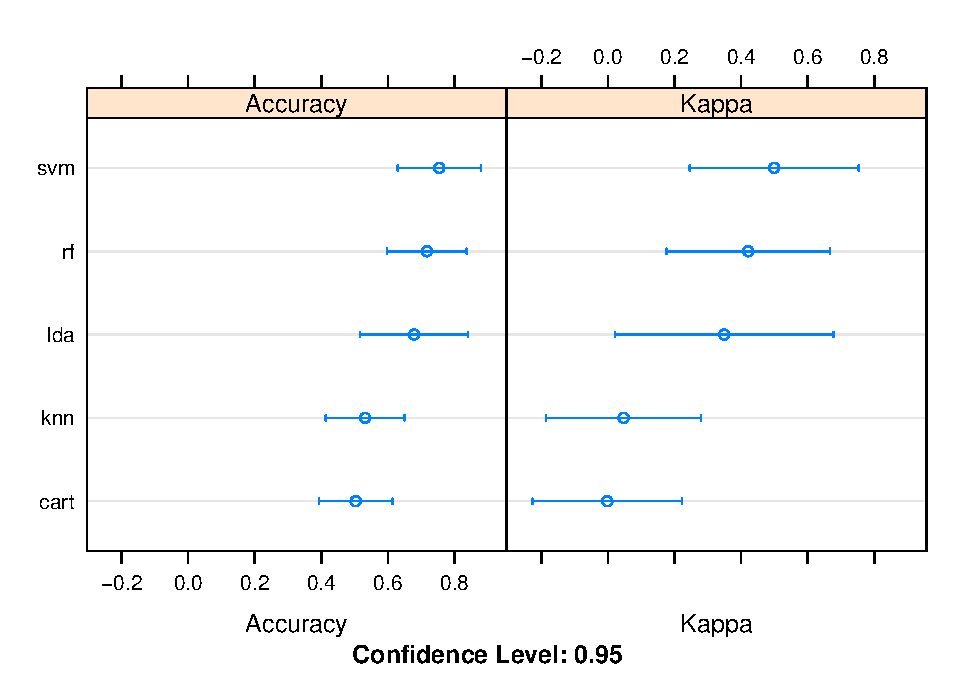
\includegraphics{heads2sem_files/figure-latex/unnamed-chunk-44-1.pdf}

summarize Best Model

\begin{Shaded}
\begin{Highlighting}[]
\KeywordTok{print}\NormalTok{(fit.rf)}
\end{Highlighting}
\end{Shaded}

\begin{verbatim}
## Random Forest 
## 
## 94 samples
##  9 predictor
##  2 classes: '1', '2' 
## 
## No pre-processing
## Resampling: Cross-Validated (10 fold) 
## Summary of sample sizes: 85, 85, 83, 84, 84, 85, ... 
## Resampling results across tuning parameters:
## 
##   mtry  Accuracy   Kappa    
##   2     0.7169697  0.4213649
##   5     0.7149495  0.4154156
##   9     0.7160606  0.4190985
## 
## Accuracy was used to select the optimal model using the largest value.
## The final value used for the model was mtry = 2.
\end{verbatim}

estimate skill of LDA on the validation dataset

\begin{Shaded}
\begin{Highlighting}[]
\NormalTok{predictions <-}\StringTok{ }\KeywordTok{predict}\NormalTok{(fit.rf, validation)}
\KeywordTok{confusionMatrix}\NormalTok{(predictions, validation}\OperatorTok{$}\NormalTok{Classification)}
\end{Highlighting}
\end{Shaded}

\begin{verbatim}
## Confusion Matrix and Statistics
## 
##           Reference
## Prediction  1  2
##          1  7  2
##          2  3 10
##                                           
##                Accuracy : 0.7727          
##                  95% CI : (0.5463, 0.9218)
##     No Information Rate : 0.5455          
##     P-Value [Acc > NIR] : 0.02455         
##                                           
##                   Kappa : 0.5378          
##                                           
##  Mcnemar's Test P-Value : 1.00000         
##                                           
##             Sensitivity : 0.7000          
##             Specificity : 0.8333          
##          Pos Pred Value : 0.7778          
##          Neg Pred Value : 0.7692          
##              Prevalence : 0.4545          
##          Detection Rate : 0.3182          
##    Detection Prevalence : 0.4091          
##       Balanced Accuracy : 0.7667          
##                                           
##        'Positive' Class : 1               
## 
\end{verbatim}

In this post you discovered step-by-step how to complete your first machine learning project in R

\hypertarget{bayes}{%
\chapter{BAYES}\label{bayes}}

\emph{Modelação Estatística Bayesiana}

\textbf{Conteúdos programáticos}

Inferência Bayesiana:

\begin{itemize}
\tightlist
\item
  Introdução à inferência Bayesiana: Probabilidade e parâmetros; Inferência frequentista clássica versus inferência Bayesiana; Fundamentos da inferência Bayesiana; Distribuições a priori; Distribuições a posteriori; Distribuições preditivas a posteriori; Modelos Bayesianos básicos; Modelação hierárquica;
\end{itemize}

Avaliação dos modelos.

\begin{itemize}
\tightlist
\item
  Construção de modelos de inferência Bayesiana: Inferência Bayesiana com distribuições a priori conjugadas; Computação Bayesiana -- métodos de Monte Carlo, métodos de Monte Carlo via Cadeias de Markov (MCMC), algoritmo de Metropolis-Hastings, algoritmo de Gibbs e outros algoritmos relacionados; Métodos de avaliação da qualidade dos modelos (escolha de valores iniciais, convergência, eficiência e precisão); Métodos de selecção de modelos; Aplicação dos métodos de inferência Bayesiana a problemas mais comuns de inferência estatística -- modelos de regressão, análise de dados categóricos e modelos de síntese de evidência.
\end{itemize}

Redes Bayesianas:

\begin{itemize}
\item
  Introdução às Redes Bayesianas: Motivação e exemplos; Probabilidade e aplicações médicas; Modelos gráficos de probabilidade; Semântica e factorização nas redes Bayesianas.
\item
  Construção de redes Bayesianas a partir de dados: Aprendizagem automática; Estimação de parâmetros de redes Bayesianas; Aprendizagem da estrutura de redes Bayesianas; Aprendizagem com dados incompletos.
\end{itemize}

\hypertarget{top}{%
\chapter{TOP.HIDA}\label{top}}

\emph{Tópicos avançados em HIDA}

\textbf{Conteúdos programáticos}

Os conteúdos abrangerão as diversas áreas da análise inteligente de dados, nomeadamente metodologias de visualização, pré-processamento, exploração e classificação de dados, proporcionando também a expansão dos conteúdos de outras UC relacionadas. A escolha dos tópicos será feita em cada edição desta unidade curricular, tendo em consideração não só o perfil e interesses dos alunos, como também os tópicos que no momento se considerem ser os mais relevantes na área.

\hypertarget{seminar1}{%
\section{Seminar 1}\label{seminar1}}

2020-02-04

\textbf{Physiological signal processing in affective computing} by Susana Brás

Susana Brás is Postdoctoral researcher at Institute of Electronics and Telematics
Engineering of Aveiro (IEETA), University of Aveiro, Portugal.
At this moment, she is focused on ECG biometric identification, emotional
modulated environments and information extraction from large biomedical databases.
Before, she was a PhD student at Abel Salazar Biomedical Sciences Institute, at
University of Porto, Portugal. Her thesis was focused on automation in anesthesia,
basically the drug distribution and effect (alterations in the brain electrical activity) were studied, modeled and a controller was presented for the hypnotic effect.
Her background is in Applied Mathematics, from the Sciences Faculty, at University of
Porto.

\hypertarget{bruno-lima}{%
\subsection{Bruno Lima}\label{bruno-lima}}

Podemos definir sinais como dados indexados a uma variável temporal e que podem ser oriundos de campos tão diversos como a biomedicina ou as comunicações sem fios.
Neste seminário foi-nos apresentado o conceito de computação afectiva que consiste em identificar emoções a partir do processamento de sinais fisiológicos. O conceito de emoção é de difícil definição ainda que a caracterização das emoções seja algo mais perceptível. Conseguimos reconhecer emoções através de respostas fisiológicas como sejam o batimento cardíaco, a expressão facial, a tensão, o riso, a rubescência ou a sudação embora estas reacções do corpo variem de pessoa para pessoa.

Com a ajuda de disciplinas como a psicofisiologia ou a psiconeuroimunologia pretende-se fazer a caracterização das emoções que permitam treinar algoritmos que identifiquem essas emoções e que assim auxiliem sistemas a tomar respostas adequadas às emoções identificadas.

O desafio é o de criar um sistema que reconheça, interprete, processe ou simule afectos humanos. Esta computação afectiva procurará ser uma ajuda perante diferentes estados emocionais. Podemos imaginar uma robot que seja de facto uma companhia para os humanos e um prestador de cuidados emocionais.
A criação de um sistema como descrito está sujeito, não só, a grandes desafios tecnológicos (como sejam: a monitorização, armazenamento, processamento, data mining e machine learning) mas também desafios éticos. Com a identificação de emoções identificam-se também preferências e consequentemente surge a possibilidade de manipular essas preferências.

No campo da saúde, a chamada \emph{`emotional analytics'} permite prever diagnósticos perante a identificação de emoções e consequentemente actuar preventivamente minimizando danos mais graves. Em campos como a saúde mental ou a saúde geriátrica a correcta classificação das emoções dos doentes é a chave para prestar os melhores cuidados de saúde.

\bibliography{book.bib,packages.bib}


\end{document}
